%=========================================================================
% (c) 2011, 2012 Josef Lusticky

\section{Network communication}
The 6LoWPAN Adaptation Layer % see Interconnecting smart objects with IP
% IEEE 802.15.4
as RFC~4944 written by 6lowpan working group of IETF
made the underlaying IEEE 802.15.4 layer
look like an IPv6 link~\cite{6lowpan} and
\begin{figure}
  \centering
  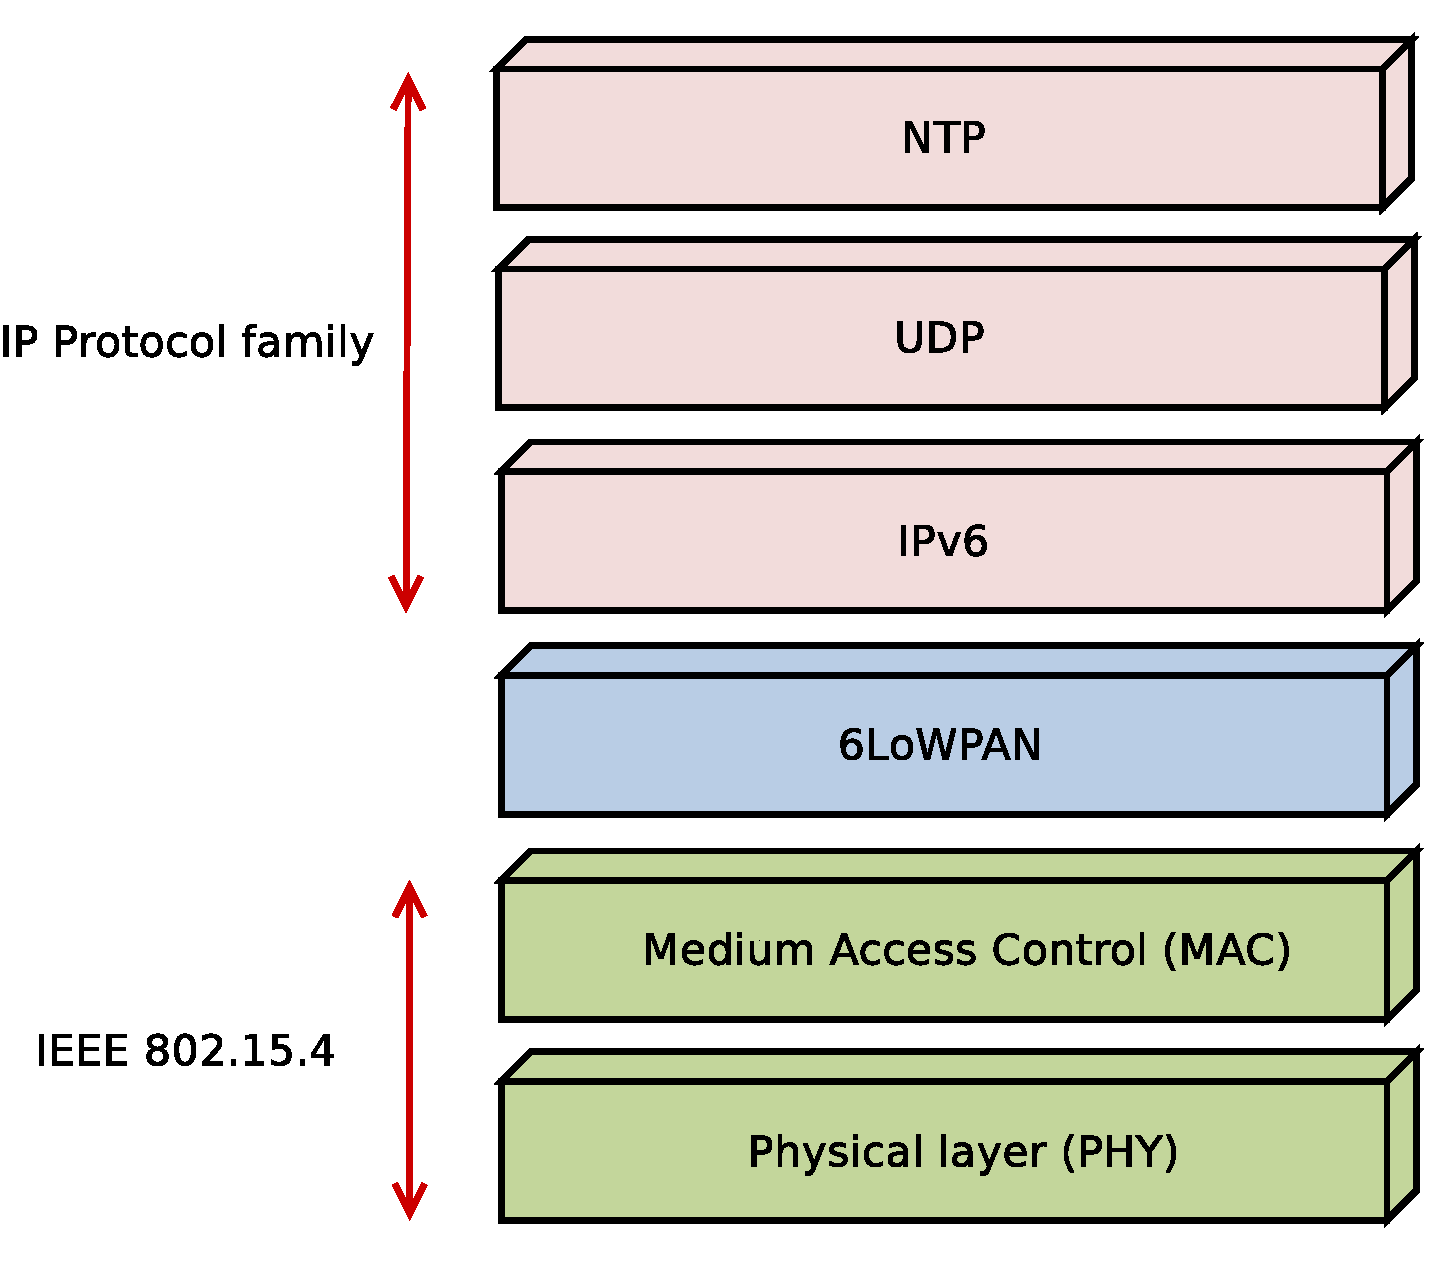
\includegraphics[width=9cm,keepaspectratio]{fig/6lowpan.pdf}
  \caption{Communication stack with 6lowpan layer}
  \label{fig:implementation-6lowpan}
  \bigskip
\end{figure}

NTP server can be specified in Makefile or
during compilate time using {\it{REMOTE\_HOST}} define.
%! TODO
TODO: If no host is specified,
NTP client assumes NTP broadcast communication mode.


% There is no IPv4 support...

%The uIP packet buffer is accessed through
%the uip\_buf array and is used to hold incoming and outgoing packets.
%The device driver should place incoming data into this buffer.
%When sending data, the device driver should read the link
%level headers and the TCP/IP headers from this buffer.
%The size of the link level headers is configured by the UIP\_LLH\_LEN
%define and in case of ethernet it is 14.

%The application data need not be placed in this buffer, so
%the device driver must read it from the place pointed to by the
%uip\_appdata pointer %as illustrated by the following example:

Routing to Meinberg NTP primary server.
Measurements made using this setup are discussed in chapter~\ref{chap:measurements}.
